%\documentstyle[epsf,twocolumn]{jarticle}       %LaTeX2e仕様
\documentclass[twocolumn]{jarticle}     %pLaTeX2e仕様(platex.exeの場合)
%\documentclass[twocolumn]{ujarticle}     %pLaTeX2e仕様(uplatex.exeの場合)

%%%%%%%%%%%%%%%%%%%%%%%%%%%%%%%%%%%%%%%%%%%%%%%%%%%%%%%%%%%%%%
%%
%%  基本バージョン
%%
%%%%%%%%%%%%%%%%%%%%%%%%%%%%%%%%%%%%%%%%%%%%%%%%%%%%%%%%%%%%%%%%
\setlength{\topmargin}{-45pt}
%\setlength{\oddsidemargin}{0cm} 
\setlength{\oddsidemargin}{-7.5mm}
%\setlength{\evensidemargin}{0cm} 
\setlength{\textheight}{24.1cm}
%setlength{\textheight}{25cm} 
\setlength{\textwidth}{17.4cm}
%\setlength{\textwidth}{172mm} 
\setlength{\columnsep}{11mm}

\kanjiskip=.07zw plus.5pt minus.5pt


% 【節が変わるごとに (1.1)(1.2) … (2.1)(2.2) と数式番号をつけるとき】
%\makeatletter
%\renewcommand{\theequation}{%
%\thesection.\arabic{equation}} %\@addtoreset{equation}{section}
%\makeatother

%\renewcommand{\arraystretch}{0.95} 行間の設定

%%%%%%%%%%%%%%%%%%%%%%%%%%%%%%%%%%%%%%%%%%%%%%%%%%%%%%%%
\usepackage[dvipdfmx]{graphicx}   %pLaTeX2e仕様(\documentstyle ->\documentclass)\documentclass[dvipdfmx]{graphicx}
\usepackage[dvipdfmx]{color}
\usepackage[subrefformat=parens]{subcaption}
\usepackage{colortbl}
\usepackage{multicol}
\usepackage{amsmath}
\usepackage{amssymb}
\usepackage{amsfonts}
\usepackage{mathbbol}

%%%%%%%%%%%%%%%%%%%%%%%%%%%%%%%%%%%%%%%%%%%%%%%%%%%%%%%%

\begin{document}

\twocolumn[
\noindent

\hspace{1em}
後期研究会発表資料2020年12月14日(月)
\hfill
\ \ 細川 岳大

\vspace{2mm}

\hrule

\begin{center}
{\Large \bf GAによる疑似ラベル探索を用いた半教師あり学習の検討}
\end{center}
\hrule
\vspace{3mm}
]

% ‚ここから 文章 Start!
\section{はじめに}
近年,機械学習は様々な分野への応用がなされており,
様々なデータセット,タスクにおいて良い性能を示している.
しかし,新規のデータセットを制作するにあたり分類タスクでは
データに対するラベル付けのコストが問題となっており,
それを解決する手法として半教師あり学習\ (Semi Supervised Learning:SSL)\ という少量のラベル付きデータからラベルなしデータに疑似ラベルを付与する手法が提案されており,
研究が盛んに研究されている.特に今年発表された\ FixMatch\cite{sohn2020fixmatch}\ という手法ではラベル付きデータが
各ラベル1枚である場合でもかなりの精度を示すことが報告されている.一方でラベル付きデータが少ないと精度のばらつきも非常に大きくなってしまう.\\
\  そこで本研究では,ラベル付きデータを遺伝的アルゴリズムで増やすことで
ラベル付きデータが非常に少ない場合における半教師あり学習の頑健性を高めることを目的とする.

\section{要素技術}
\subsection{FixMatch}
FixMatch\cite{sohn2020fixmatch}\ は\ SSL\ の一つである.
図\ref{fig:daigram1}に\ FixMatch\ 概略図を示す.
\begin{figure}[h]
	\begin{center}
		\vspace*{-3mm}
		\hspace*{-8mm}
		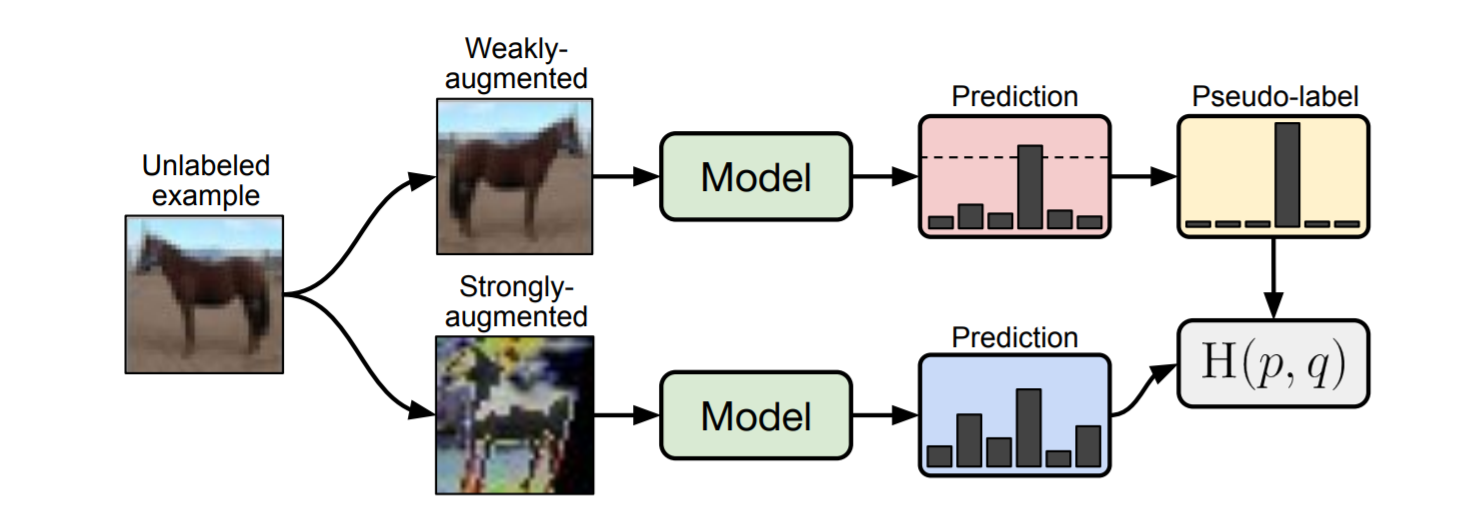
\includegraphics[height=40mm,width=100mm]{1.PNG}
		\caption{FixMatch\cite{sohn2020fixmatch}の概略図\label{fig:daigram1}}
	\end{center}
\end{figure}

この手法は\ Pseudo\ Label\ (疑似ラベル)と\ Consistency\ Regularization\ の統合した手法である.疑似ラベルはラベル付きデータから生成されたモデルに対しラベルなしデータを入力としたときの出力のうち最も確信度の高いラベルをそのデータのラベルとするものであり,\ Consistency\ Regularization\ は画像データに変換をかける前後において出力値が変化しないような制約をかける正則化手法である.\\
\ FixMtach\ におけるラベル付きデータのバッチサイズを\ $B$\ ,ラベルなしデータのバッチサイズを$\mu B$とする.$p_{\rm m}(y|x)$を入力$x$に対するモデルの出力,
${\rm H}(p, q)$を確率分布$p,q$に対する\ Cross\ Entropy\ Loss\ する.また,画像の弱変換,強変換をそれぞれ$\alpha(\cdot),初期{\cal A}(\cdot)$とすると,\ FixMatch\ の\ loss\ は(\ref{quad5})式となる.
 \begin{eqnarray}
 \label{quad1}
 l_{\rm s} = \frac{1}{B}\sum^{B}_{b=1}{\rm H}(p_b,p_{\rm m}(y|\alpha(x_b)))\\
 \label{quad2}
 q_b = p_{\rm m}(y|\alpha(u_b))\\
 \label{quad3}
 \hat{q}_b = {\rm argmax}(q_b)\\
 \label{quad4}
 l_{\rm u} = \frac{1}{\mu B}\sum^{\mu B}_{b=1}
 {\mathbb{1}({\rm max}(q_b)\geq\tau){\rm H}(\hat{q}_b,p_{\rm m}(y|{\cal A}(u_b)))}\\
 \label{quad5}
 loss_{\rm total} = l_{\rm s} + \lambda \,l_{\rm u}
 \end{eqnarray}
 このとき$\tau$は確信度の閾値であり$\lambda$はラベルなしデータにおける\ loss\ の重みである.
\ref{quad1}式はラベル付きデータに対する\ loss\ であり,
\ref{quad2}式は弱変換後のラべうなしデータに対する\ model\ の予測,
\ref{quad3}式の$hat{q}_b$ は疑似ラベル,
\ref{quad4}式はラベルなしデータに対する\ loss\ であり,\ref{quad1}式と比較して
弱変換が強変換に,確信度が低いものにマスクをかける関数が組み込まれている違いがある.

\subsection{遺伝的アルゴリズム}
遺伝的アルゴリズム(Genetic Algorithm:GA)\cite{whitley1994genetic}とは生
物の進化を模倣して適切なデータを見つけるアル
ゴリズムである.最小単位を遺伝子とし,探索する
データを遺伝子の集合である個体として表現する.
各個体の適応度を計算し,個体の集まりである集団に対し
選択,交叉,突然変異の三種類の操作を適用させ次の集団を作る,
という操作を繰り返して適応度の高い個体を探索する.
交叉の特性上,他のアルゴリズムより局所探索になりにくいが,
一方で設定によっては初期収束を起こしてしまう.
\section{データセット}
データセットについて\ CIFAR-10\ を用いた.\ CIFAR-10\ は6万枚の画像からなる
データセットであり,各画像 32×32 pixel のカラー画像でそれぞれに\{airplane, automobile, bird, cat, deer, dog, frog, horse, ship, truck\}の10種類のラベルがついている.
\section{提案手法}
今回はFixMatch\ に\ GA\ を導入した手法について提案する.
\begin{enumerate}
	\item データをラベル付きデータ(:$D_{\rm L}$),ラベルなしデータ(:$D_{\rm {NL}}$), 探索データ(:$D_{\rm S}$),テストデータ(:$D_{\rm T}$)に分割する.
	\item $D_{\rm L}$の一部の$D_{\rm {NL}}$を用いて\ FixMatch\ により\ model\ を学習させる
	\item 生成された\ model\ から探索データに仮のラベルを付け,\ GA\ の初期個体のベースとし,手順2での未使用のラベルなしデータの\ error\ 率で各遺伝子座ごとに突然変異させて初期個体を得る.
	\item 得られた初期個体から\ GA\ を回す.
	\item 最終的に得られた個体を探索データに対するラベルとみなし,ラベル付きデータに追加し\ FixMatch\ で再学習しテストデータに対する精度を求める.
\end{enumerate}

\subsection{GA の設定}
\subsubsection{個体表現}
各遺伝子はラベルなしデータに対する\ CIFAR-10\ のラベルデータである0 $\sim$ 9までのいずれかの整数値を持つ.全個体を通して各遺伝子座に対する探索データが共通であり一意に決まっているため,
個体の遺伝子長は探索するデータ数となる.

\subsubsection{選択}
選択手法はエリート選択とトーナメント選択を用いた.エリート選択は前世代における最大の適応度を持つ個体を必ず次の世代に残す手法で本実験では毎世代2つ選択する.トーナメント選択はランダムに複数の個体を選びそのうちで最も高い適応度を持つものを選択する方法である.なお,ランダムに選ぶ個数をトーナメントサイズと呼び,本実験では3に設定した.

\subsubsection{交叉}
交叉手法は二点交叉を用いた.二点交叉とは,交叉する2つの個体を三分割し,それぞれの部分の遺伝子らを入れ替える手法である.

\subsubsection{突然変異}
突然変異はある遺伝子に対し他の対立遺伝子へとランダムに変更するものとした.また突然変異率について各遺伝子座に対し5\%でほかのラベルに変化するものとした.

\section{数値実験}
半教師あり学習のタスクとして,本実験では\ cifar10\ の\ train\_data\ 50000枚のうちラベル付きデータを各ラベル25枚,計250枚のみを用いるタスクで実験した.また今回探索するデータについて,ランダムな選択ではあるものの,各正答ラベルが均等になるように選ばれている.
表\ref{tb:FTXpara},\ref{tb:GApara}に実験設定を示す.
\begin{table}[h]
	\centering
	\caption{FixMatchの設定\label{tb:FTXpara}}
	\scalebox{1.1}{
		\begin{tabular}{|c|c|c|} \hline
			model&\multicolumn{2}{c|}{WideResNet16-2}\\ \hline\hline
			data set&\multicolumn{2}{c|}{CIFAR-10}\\ \hline
			batch size&labeled&32\\ \cline{2-3}
			&unlabeled&$32 \times 7$\\ \hline
			optimizer&\multicolumn{2}{c|}{SGD(lr=0.1,momntum=0.9)}\\ \hline\hline
			\multicolumn{3}{|c|}{事前学習}\\ \hline
			train &labeled&100\\ \cline{2-3}
			&unlabeled&49650\\ \hline			
			val data&\multicolumn{2}{c|}{150}\\ \hline
			num\_iterations&\multicolumn{2}{c|}{2\textasciicircum 15}\\ \hline\hline
			\multicolumn{3}{|c|}{個体の適応度の評価}\\ \hline
			train &searchのみ&100\\ \cline{2-3}
			&unlabeled&49650\\ \hline
			val data&\multicolumn{2}{c|}{250}\\ \hline
			num\_iterations&\multicolumn{2}{c|}{5000}\\ \hline\hline
			\multicolumn{3}{|c|}{得られた個体の評価}\\ \hline
			train &labeled+search&250+?\\ \cline{2-3}
			&unlabeled&49650\\ \hline	
			val data&\multicolumn{2}{c|}{10000}\\ \hline
			num\_iterations&\multicolumn{2}{c|}{2\textasciicircum 16}\\ \hline
		\end{tabular}
	}
\end{table}

\begin{table}[h]
	\centering
	\caption{GAの設定\label{tb:GApara}}
	\scalebox{1.0}{
		\begin{tabular}{|c||c|} \hline
			個体数&20\\ \hline
			世代数&20\\ \hline
			交叉率&1.0\\ \hline
			突然変異率&0.05\\ \hline\hline
			labeled&250枚\\ \hline
			search&100枚\\ \hline
		\end{tabular}
	}
\end{table}

\section{実験結果および考察}
図\ref{fig:ex1},\ref{fig:ex1_1}に実験結果を示す.
図\ref{fig:ex1}について箱ひげ図は各個体の適応度を示しており,折れ線グラフは各世代における探索データに対する正解ラベルの最大と平均の割合を示しており,共に左の数値に従っている.また横軸は世代数となっている.図\ref{fig:ex1_1}は縦軸が適応度,横軸が個体の正解ラベルに対する割合となっており,探索された全個体についての散布図である.\\
\ \ \ 図\ref{fig:ex1}より最大正答数の増加は見られないが平均の正答数は上がっていることは確認できる.また,適応度としても収束しつつあり,これ以上の精度改善は困難であると思われる.また図からは読み取ることはできないが,各世代の適応度最高値は正答数が多いものだけに関わらず,特に正答数の低いものも選ばれることも多々あった.これはデータ数が非常に少ないことが大きな原因であることが考えられる.さらに12世代以降で最大及び平均の正答数が減っていることもわかる.これは過学習と同様に250枚という少ないデータに適合しすぎて汎化性が失われていると考えられる\\
\ \ \ 図\ref{fig:ex1_1}から相関性はありそうではあるが,実際には学習が全く進んでいない.これは先にも述べた通りデータの少なさゆえに正答数に対して適応度に幅が出てしまっているからであることが分かる.\\ 
\begin{figure}[h]
	\begin{center}
		\vspace*{-3mm}
		\hspace*{-8mm}
		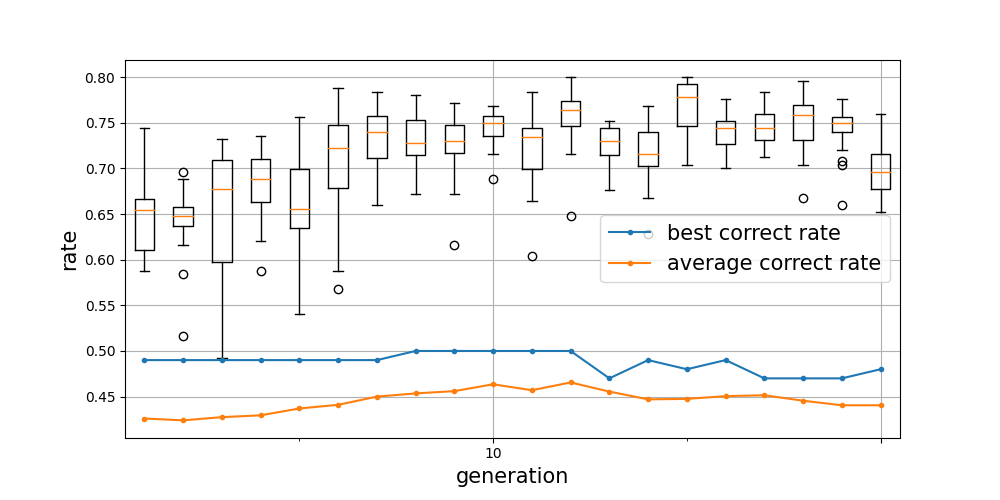
\includegraphics[height=70mm,width=100mm]{graph.png}
		\caption{実験の結果\label{fig:ex1}}
	\end{center}
\end{figure}
\begin{figure}[h]
	\begin{center}
		\vspace*{-3mm}
		\hspace*{-8mm}
		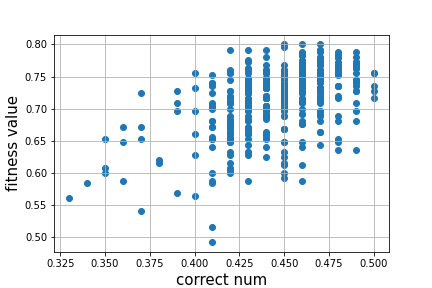
\includegraphics[height=70mm,width=100mm]{img.png}
		\caption{実験の相関図\label{fig:ex1_1}}
	\end{center}
\end{figure}

また表\ref{tb:ex1}に適応度の平均が最高であった14世代の個体を用いて再学習した結果を示す.採択される遺伝子はある遺伝子座を全個体通してみた時に最も多く出現した遺伝子とする.閾値はある遺伝子座において採択された遺伝子の出現数が全個体に対して占めていた割合に対するものである.\\
\ \ \ 結果としてラベル付きデータのみを用いたものを超えることはできない結果となった.従来のシンプルな疑似ラベルを追加する手法\cite{lee2013pseudo}において疑似ラベルの役割としてエントロピーの正則化が挙げられている.つまり\ FixMatch\ における正則化が強く,探索されたデータの疑似ラベルの正則化がうまく働かず,探索を阻害したと考えられる.\\
\ \ 結論として,データが少ない状況において\ cifar10\ といった画像データかつ10種類の分類タスクにおけるラベル付けは今回の設定の\ GA\ の学習でほとんど得られないことが分かった.

\begin{table}[h]
	\centering
	\caption{GA\ の設定\label{tb:ex1}}
	\scalebox{1.0}{
		\begin{tabular}{|c|c|c|c|} \hline
			採択数&正答数&閾値&精度\\ \hline
			0&&&0.868\\ \hline\hline
			100&46&なし&0.836\\ \hline
			39&22&0.19&0.862\\ \hline
			19&14&0.2&0.825\\ \hline
		\end{tabular}
	}
\end{table}

\section{まとめと今後の課題}
 本研究からGAによるラベルなしデータのラベル付けを提案した.
 しかし,結果として\ GA\ で得られた疑似ラベルによって\ FixMatch\ の精度改善にはつなげることはできなかった.ただしデータとしての正答数の平均自体の改善はみられるため\ FixMatch\ の\ loss\ として\ GA\ のような動作を組み込むことができればと考えている.
 また,近年の半教師あり学習において自己教師あり学習を組み込んだもの\cite{chen2020simple,wang2019enaet}がより成果を出しており,今後の課題としてそれらに\ GA\ が適用できないかということがあげられる.

\bibliographystyle{unsrt}
\bibliography{sa}


\end{document}


